% =====================================================================
% THIS FILE IS THE SOURCE. Edit it, then rebuild the PDF with:
%     bash tools/compile.sh Unit_05_Regression_as_Reasoning
% (run from the Course_Rewrite folder; it compiles twice and reports
%  page count, overfull boxes, and em dashes)
%
% Do not edit the PDF directly. Figures are the fig_*.pdf files in this
% folder, regenerated by tools/make_module*_slide_figs.py.
%
% Originally converted from the 15-module draft by a one-shot script now
% parked in tools/one_shot_generators/. Re-running those would discard
% anything you change here, so they are kept out of tools/ on purpose.
% =====================================================================
\documentclass[aspectratio=169]{beamer}
\usetheme{default}
\usefonttheme{professionalfonts}
\usepackage{amsmath, amssymb, amsfonts}
\usepackage{graphicx}
\usepackage{booktabs}
\usepackage{bm}
\usepackage{hyperref}

\mode<presentation> {
    \usetheme{Frankfurt}
    \usecolortheme{default}
}

% == notation shortcuts ==
\newcommand{\xbar}{\bar{x}}
\newcommand{\SE}{\mathrm{SE}}
\newcommand{\se}{\widehat{\SE}}
\newcommand{\Hzero}{H_0}
\newcommand{\Hone}{H_1}

% Recurring motifs (color-coded). Frankfurt: block=blue, alert=red, example=green.
\newenvironment{principle}[1]{\begin{block}{\textbf{Principle:} #1}}{\end{block}}
\newenvironment{trap}[1]{\begin{alertblock}{\textbf{Trap:} #1}}{\end{alertblock}}
\newenvironment{practice}[1]{\begin{exampleblock}{\textbf{In practice:} #1}}{\end{exampleblock}}
\newenvironment{interview}[1]{\begin{exampleblock}{\textbf{You may be asked:} #1}}{\end{exampleblock}}
\newenvironment{yourturn}[1]{%
  \setbeamercolor{block title}{fg=white,bg=orange!80!black}%
  \setbeamercolor{block body}{bg=orange!12}%
  \begin{block}{\textbf{Your turn:} #1}}{\end{block}}
\newenvironment{livedemo}[1]{%
  \setbeamercolor{block title}{fg=white,bg=teal!80!black}%
  \setbeamercolor{block body}{bg=teal!12}%
  \begin{block}{\textbf{Live demo:} #1}}{\end{block}}
% "LLM check" mistake-or-not exercise (violet, locally colored).
\newenvironment{llmcheck}[1]{%
  \setbeamercolor{block title}{fg=white,bg=violet!75!black}%
  \setbeamercolor{block body}{bg=violet!10}%
  \begin{block}{\textbf{LLM check:} #1}}{\end{block}}

\title{Regression as Reasoning}
\subtitle{Unit 5: Reasoning With a Slope}
\author{Stat 220 \textbar{} Statistics for Data Science}
\date{}

\begin{document}

\begin{frame}
  \titlepage
\end{frame}

% ======================================================================
\section{Why}
% ======================================================================
\begin{frame}{Where we left off}
\begin{itemize}
  \item In Part 1 we learned to judge a single estimate against its noise, using the template
        $(\text{estimate}-\text{null})/\se$.
  \item Regression is the same idea, but now the estimate we care about is a \textbf{slope}:
        how much $y$ changes as $x$ changes.
  \item Everything you already know comes back: standard errors, $p$-values, confidence
        intervals, and the same traps. We're just pointing them at a more useful question.
\end{itemize}
\begin{principle}{the bridge}
A regression slope is an estimate with a standard error, exactly like a sample mean. So we get
to reuse the entire toolkit from Part 1.
\end{principle}
\end{frame}

\begin{frame}{Why regression runs data science}
\begin{itemize}
  \item It does \textbf{two jobs at once}: it \emph{predicts} ($\hat{y}$ for a new case) and it
        \emph{explains} (how $y$ relates to each $x$).
  \item Almost every model you'll meet, from a simple line to a deep network, is some
        descendant of ``draw the best relationship between inputs and an output.''
  \item And the interesting questions aren't about the formula. They're about which variables
        belong in the model, and what a coefficient really means once they're there.
\end{itemize}
\begin{practice}{the shape of this module}
``You added a variable and another coefficient flipped sign. Which number do you believe, and
why?''
\end{practice}
\end{frame}

\begin{frame}{What this unit gives you}
\begin{columns}[T]
\begin{column}{0.5\textwidth}
\textbf{Things to know}
\begin{itemize}\small
  \item what a regression line is, and what least squares actually minimizes
  \item how to read a slope and an intercept \emph{with their units}
  \item that a slope is an estimate, so it carries a standard error
  \item how binary and categorical predictors enter a model
  \item what an interaction means, in words
  \item what happens to a coefficient when you add or remove another predictor
\end{itemize}
\end{column}
\begin{column}{0.5\textwidth}
\textbf{Mistakes to stop making}
\begin{itemize}\small
  \item reading a slope without checking its units or its range
  \item treating a slope as the effect of intervening
  \item confusing a significant slope with a useful model
  \item chasing $R^2$ as if it measured correctness
  \item comparing coefficients on variables measured in different units
  \item controlling for a variable without asking what it does in the causal story
\end{itemize}
\end{column}
\end{columns}
\end{frame}

% ======================================================================
\section{Activity}
% ======================================================================
\begin{frame}{Live experiment: the magic feather}
\vfill
\begin{livedemo}{I need 10 volunteers}
\centering
\Large Ten volunteers, one bottle each.
\end{livedemo}
\vfill
\end{frame}

\begin{frame}{Read the board before you explain it}
Two columns of numbers are now on the board. Three questions, in this order.
\begin{enumerate}
  \item \textbf{What did the coached three do?} Compare their round 2 to their round 1.
  \item \textbf{What did the top three do?} They got no pep talk, no feather, and no attention.
        They are the comparison group, and they are the whole point.
  \item \textbf{What did the middle four do?}
\end{enumerate}
\begin{trap}{the objection to raise yourself}
The bottom three started near zero, so they had more room to go up than down. That is a real
criticism of the comparison. It is also exactly why we look at the top three, who had room in
both directions and nobody coaching them.
\end{trap}
\end{frame}

\begin{frame}{Two things that are true whatever the bottles did}
\begin{principle}{regression to the mean}
When you pick people out on an extreme score, some of what made that score extreme was skill and
some was luck. Skill shows up again next time. Luck does not. So a group selected at either end
drifts back toward the middle on its own, with nothing done to it and nobody helping.
\end{principle}
\begin{principle}{a predictor can be real and still be circumstantial}
``Received the pep talk'' would predict improvement here. It would sit in a regression with a
positive coefficient and a small $p$-value. It would still not be doing anything. It predicts
because of \emph{how the group was chosen}, not because of what was done to them.
\end{principle}
\centering\small
The rest of this unit is about telling those two apart in data where nobody knows the answer.
\end{frame}

\begin{frame}{Where the word ``regression'' comes from}
\begin{itemize}
  \item Francis Galton, 1886, measuring the heights of parents and their grown children.
  \item Tall parents had tall children, but on average \textbf{closer to the middle} than the
        parents were. Same for short parents in the other direction.
  \item He called it \emph{regression toward mediocrity}, and that phrase is why the technique
        this entire unit is about is called \textbf{regression}.
\end{itemize}
\begin{principle}{what Galton nearly got wrong}
He first read it as a force pulling humanity toward the average. It is not a force. It is what
happens to any measurement that is part skill and part luck, which is nearly all of them.
\end{principle}
\centering\small
You just ran his experiment with water bottles.
\end{frame}

\begin{frame}{Live experiment: guess the correlation}
\begin{livedemo}{a quick contest}
Below are four scatterplots, A through D. For each one, \textbf{write down your guess} for the
correlation: a single number between $-1$ and $+1$.
\end{livedemo}
\vspace{0.2em}
{\tiny\textit{Materials: none. Time: 6 minutes.}}
\centering
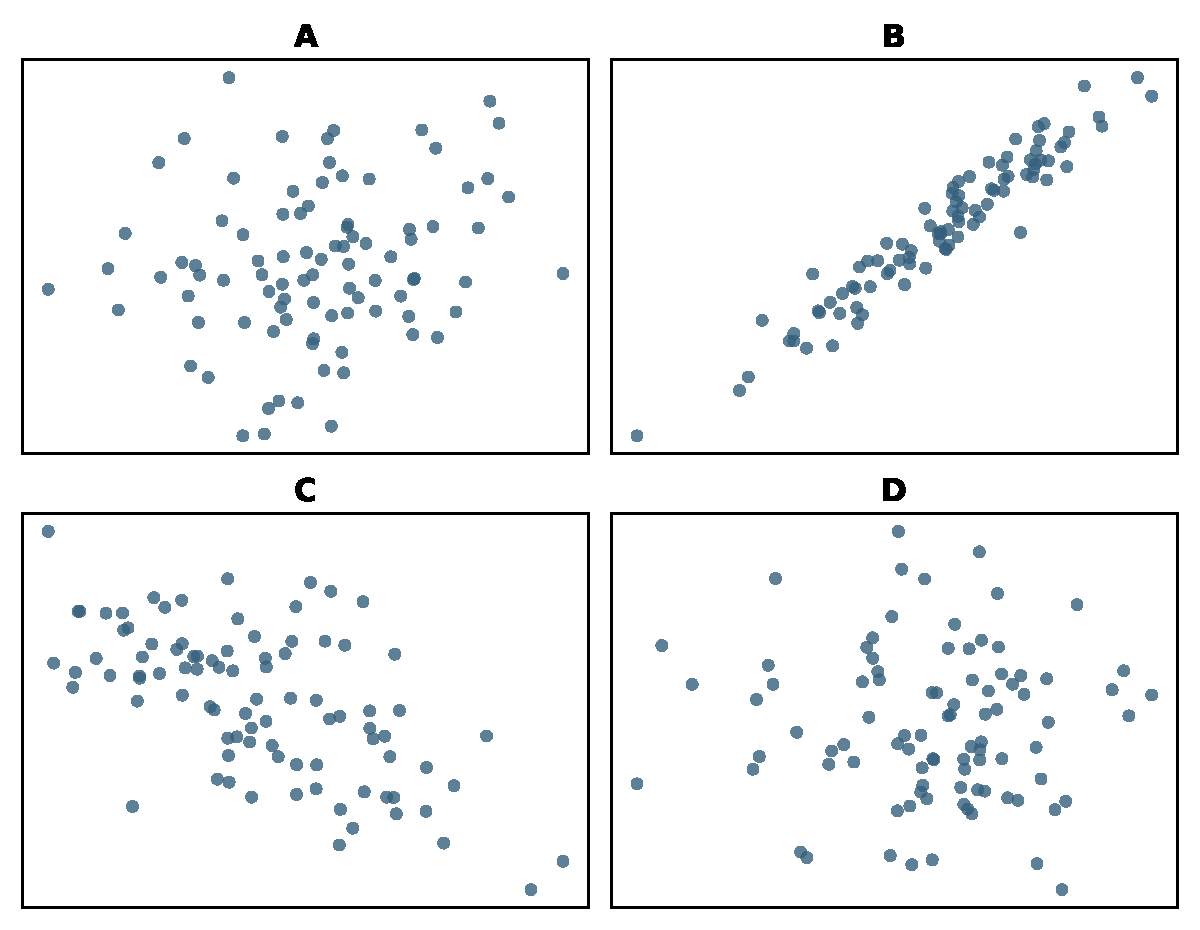
\includegraphics[height=0.5\textheight]{fig_guess_correlation.pdf}\\[2pt]
\small Closest set of four guesses wins. We'll call on a few of you to defend a number.
\end{frame}

\begin{frame}{Guess the correlation: the reveal}
\begin{columns}[c]
\begin{column}{0.6\textwidth}
\centering
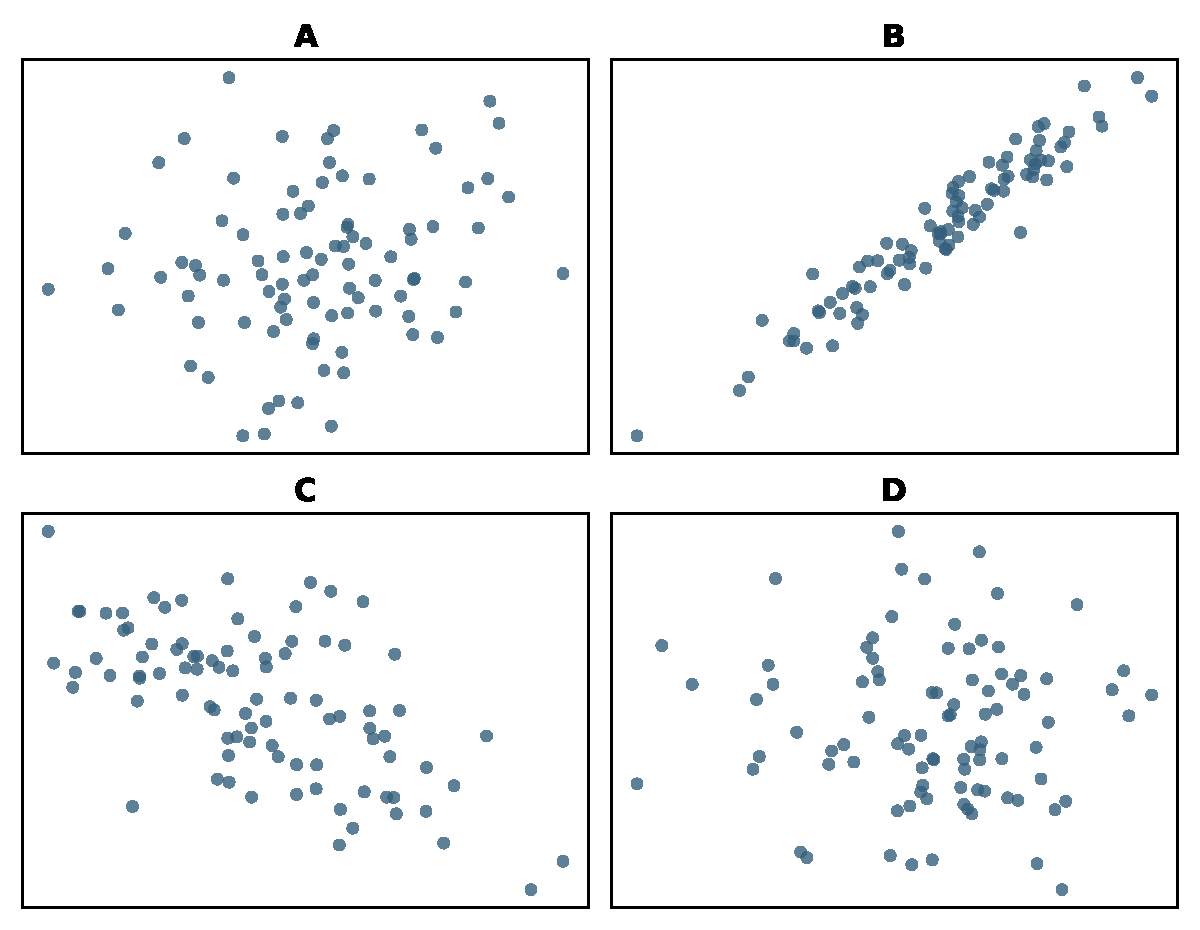
\includegraphics[width=\textwidth]{fig_guess_correlation.pdf}
\end{column}
\begin{column}{0.4\textwidth}
\small
The true correlations:
\begin{itemize}
  \item A: $r \approx 0.2$ (weak)
  \item B: $r \approx 0.96$ (very strong)
  \item C: $r \approx -0.6$ (moderate, negative)
  \item D: $r \approx 0.0$ (basically none)
\end{itemize}
\vspace{0.4em}
Eyeballing is hard, and a vibe is not a number. Regression gives us the number, and the line
that goes with it.
\end{column}
\end{columns}
\end{frame}

\begin{frame}{The arc of an analysis: from question to answer}
Almost every regression analysis follows the same order, and the order matters more than the
syntax:
\begin{enumerate}
  \item \textbf{Pin down the question.} Predict, or explain? Whose effect do you actually care about?
  \item \textbf{Know the data.} What is each variable, in what units, and how was it collected
        (assigned in an experiment, or just observed)?
  \item \textbf{Look first.} Plot it. Check the range, the outliers, and any obvious lurking variable.
  \item \textbf{Build the model the question needs.} Which predictors belong, and why each one?
  \item \textbf{Check it.} Residuals, and the assumptions from Part 1.
  \item \textbf{Read the answer.} The coefficient as a sentence, its uncertainty, and the
        caveats: confounding, extrapolation, causal or not.
\end{enumerate}
\end{frame}

% ======================================================================
\section{The line}
% ======================================================================
\begin{frame}{What regression actually is}
\begin{columns}[c]
\begin{column}{0.56\textwidth}
\centering
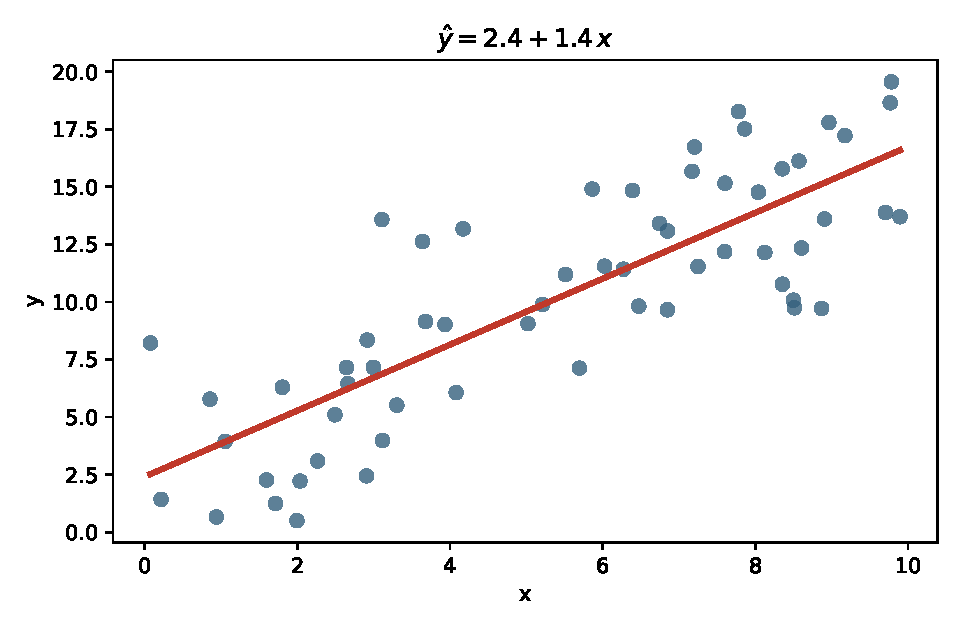
\includegraphics[width=\textwidth]{fig_reg_scatter.pdf}
\end{column}
\begin{column}{0.44\textwidth}
\small
We draw the line that fits the cloud best:
\[
   \hat{y} \;=\; b_0 + b_1\,x .
\]
\begin{itemize}
  \item $b_0$ (intercept): predicted $y$ when $x=0$.
  \item $b_1$ (slope): how much $\hat{y}$ moves when $x$ goes up by one unit.
\end{itemize}
That single number $b_1$ is usually the thing you actually care about.
\end{column}
\end{columns}
\end{frame}

\begin{frame}{Reading the slope and intercept (mind the units)}
\begin{itemize}
  \item A slope always carries units: ``\emph{units of $y$} per one \emph{unit of $x$}.''
  \item ``$b_1 = 1.7$'' is meaningless until you say ``1.7 \emph{inches of height} per one
        \emph{shoe size}.''
  \item The intercept is only meaningful if $x=0$ is meaningful. A predicted height at shoe
        size 0 is nonsense, and that is fine. The intercept only positions the line.
\end{itemize}
\begin{principle}{interpretation is a sentence, not a number}
Always state a slope as a full sentence with units and direction: ``each extra X is associated
with $b_1$ more Y.'' If you can't say the sentence, you don't understand the model yet.
\end{principle}
\end{frame}

\begin{frame}{Reading a fitted line out loud}
Suppose a fit on housing data gives
\[
\widehat{\text{price}} = 41{,}000 + 118 \times \text{square feet}.
\]
\begin{itemize}
  \item \textbf{Slope:} each extra square foot is associated with \$118 more in price,
        \emph{among houses like these}. Units: dollars per square foot.
  \item \textbf{Intercept:} the fitted price of a zero-square-foot house. Not a house. Intercepts
        are often meaningless alone. They position the line.
  \item \textbf{Range matters:} if the data runs 800 to 3{,}000 square feet, the line says nothing
        about a 12{,}000-square-foot mansion.
\end{itemize}
\begin{trap}{the units trap}
``The coefficient is 118, so it is a big effect.'' Big compared to what? Switch to square
\emph{meters} and the same relationship reports 1{,}270.
\end{trap}
\end{frame}

\begin{frame}{Residuals and least squares}
\begin{columns}[c]
\begin{column}{0.56\textwidth}
\centering
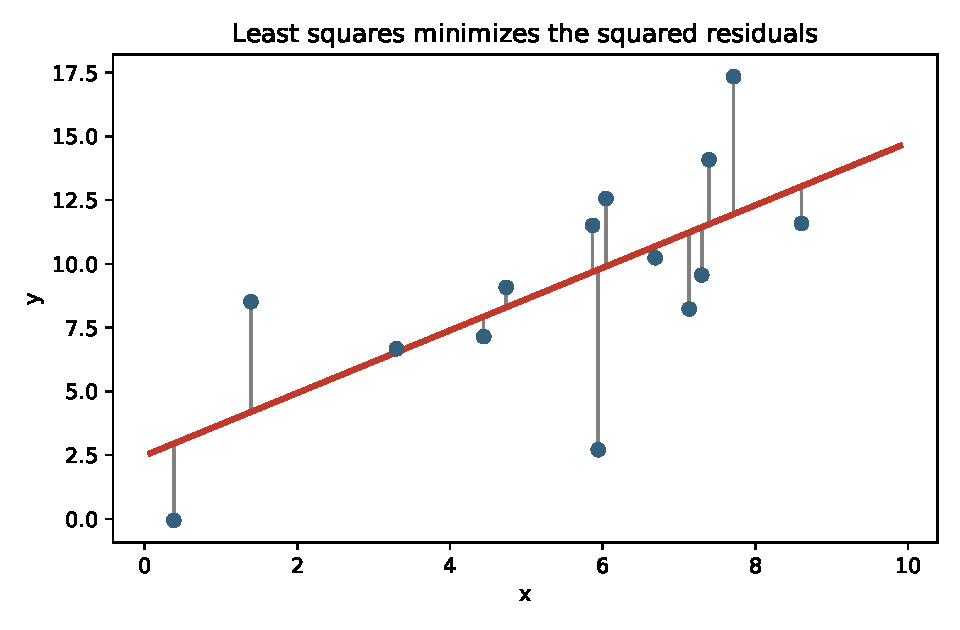
\includegraphics[width=\textwidth]{fig_reg_residuals.pdf}
\end{column}
\begin{column}{0.44\textwidth}
\small
\begin{itemize}
  \item A \textbf{residual} is the vertical gap between a point and the line: what the model
        missed for that case.
  \item ``Least squares'' picks the line that makes the sum of \emph{squared} residuals as
        small as possible.
  \item Squaring is why a few far-off points (outliers) can pull the line toward them.
\end{itemize}
\end{column}
\end{columns}
\end{frame}

\begin{frame}{A slope is an answer to a question}
\begin{itemize}
  \item ``Does price go up with size?'' The slope answers it, with a sign and a magnitude.
  \item ``How much more do customers spend per extra email?'' The slope answers it.
  \item Prediction uses the whole line. Explanation usually lives in a single slope.
\end{itemize}
\begin{principle}{keep the question in view}
Before you read any coefficient, say the question it answers out loud. The math is the easy
part. Knowing which slope answers your question is the skill.
\end{principle}
\end{frame}

\begin{frame}{Your turn \#1}
\begin{yourturn}{say the sentence}
A coffee chain fits
\[
   \widehat{\text{daily sales}} \;=\; 480 + 32\,(\text{loyalty emails sent}).
\]
\vspace{0.2em}
Turn to a neighbor and practice explaining, in one clear sentence with units, what the
\textbf{32} means. Then: would you keep sending emails forever?
\end{yourturn}
\end{frame}

\begin{frame}{Your turn \#1: answer}
\begin{itemize}
  \item ``Each additional loyalty email is associated with about \textbf{\$32 more} in
        predicted daily sales.'' Units and direction, in a sentence.
  \item ``Forever?'' No. The data only covers the range we actually observed. Pushing $x$ far
        past that is \alert{extrapolation}, and the line has no idea what happens out there.
\end{itemize}
\begin{principle}{a slope is local}
A linear fit describes the relationship \emph{inside the range of your data}. Read it there,
not in a fantasy world far outside it.
\end{principle}
\end{frame}

% ======================================================================
\section{Inference on a slope}
% ======================================================================
\begin{frame}{The slope is an estimate, so it has a standard error}
\begin{itemize}
  \item Run the study again with new data and you'd get a slightly different slope. So $b_1$ is
        a random quantity with a sampling distribution, just like a mean.
  \item Its spread is $\se(b_1)$, and the familiar template comes right back:
\end{itemize}
\[
   t \;=\; \frac{b_1 - 0}{\se(b_1)} .
\]
\begin{principle}{same engine, new question}
Testing a slope is the Coke test again: assume the slope is really 0 (``$x$ doesn't matter''),
then ask how surprising a slope this big would be.
\end{principle}
\end{frame}

\begin{frame}{Testing whether the slope is zero}
\begin{itemize}
  \item \textbf{Null:} $b_1 = 0$, meaning $x$ has no linear relationship with $y$.
  \item The software hands you $b_1$, its SE, the $t$, and a $p$-value. The $p$-value means
        exactly what it did in Part 1: how surprising this slope would be if the true slope
        were 0.
  \item For our scatter: $b_1 = 1.43$, $\se = 0.13$, so $t \approx 11$ and $p$ is tiny. The
        upward relationship is not a fluke.
\end{itemize}
\begin{practice}{say it cleanly}
``A small $p$ on the slope says the relationship is hard to explain by chance. It does not say
the relationship is large or useful. That's a separate question.''
\end{practice}
\end{frame}

\begin{frame}{The same traps come back}
\begin{itemize}
  \item With enough rows, a slope of essentially zero can still be ``highly significant.''
        Significance is partly a statement about your sample size.
  \item A confidence interval for the slope is almost always the better thing to report:
        $b_1 \pm (\text{critical } t)\times \se(b_1)$.
\end{itemize}
\begin{trap}{$R^2$ is not significance, and significance is not importance}
A slope can have $p < 0.001$ and an $R^2$ of $0.01$: a real relationship that explains almost
none of the variation. Significant and important are different words.
\end{trap}
\end{frame}

\begin{frame}{Scenario: significant slope, tiny $R^2$}
\textbf{Setup.} On 200{,}000 customers, ``ads seen'' predicts ``spending'' with $p < 10^{-9}$,
slope $= \$0.02$ per ad, and $R^2 = 0.004$.
\begin{itemize}
  \item The relationship is real (huge sample, tiny $p$) but explains almost nothing, and the
        per-ad effect is two cents.
  \item ``Significant'' here is mostly a story about having 200{,}000 rows.
\end{itemize}
\begin{practice}{how to answer}
``It's a real but tiny relationship. I'd report the effect size and CI, note that $R^2$ is
near zero so ads barely move spending, and let the business decide if two cents an ad is worth
it.''
\end{practice}
\end{frame}

% ======================================================================
\section{Binary and categorical}
% ======================================================================
\begin{frame}{A 0/1 predictor: the dummy variable}
\begin{columns}[c]
\begin{column}{0.56\textwidth}
\centering
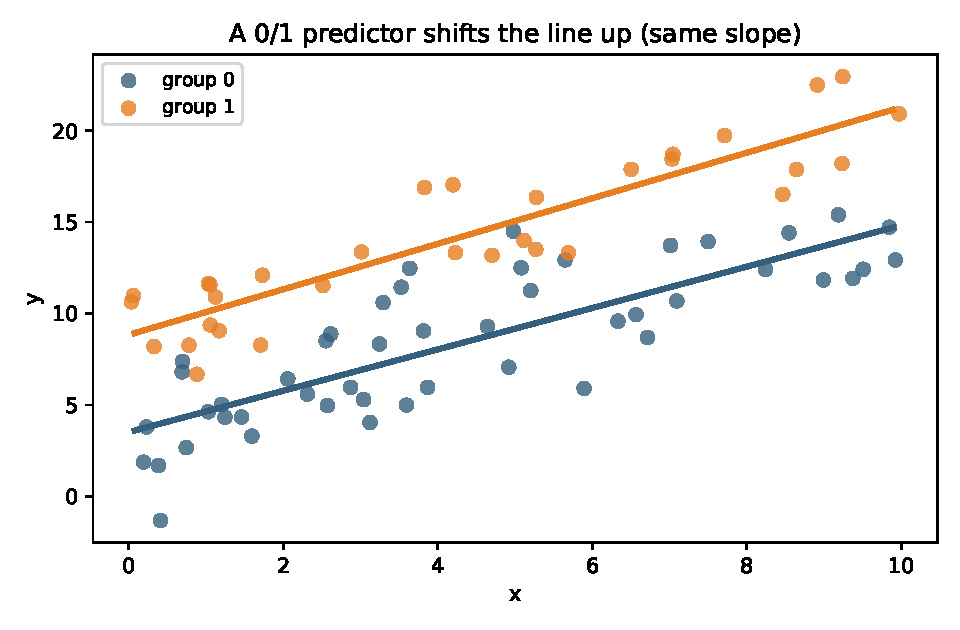
\includegraphics[width=\textwidth]{fig_dummy.pdf}
\end{column}
\begin{column}{0.44\textwidth}
\small
Code a yes/no variable as 1/0 and drop it in the model:
\[
   \hat{y} = b_0 + b_1 x + b_2\,(\text{group}).
\]
\begin{itemize}
  \item $b_2$ shifts the whole line up or down.
  \item You get two \textbf{parallel} lines, one per group.
  \item $b_2$ is the gap between them, holding $x$ fixed.
\end{itemize}
\end{column}
\end{columns}
\end{frame}

\begin{frame}{The dummy coefficient is a group comparison}
\begin{itemize}
  \item $b_2$ answers: ``at the same $x$, how much higher is group 1 than group 0?''
  \item With no $x$ in the model at all, that coefficient is just the difference in group means.
        It is the two-sample comparison from Unit 1, written as a regression.
\end{itemize}
\begin{principle}{regression unifies the tests}
A two-group $t$-test is a regression on a single 0/1 predictor. Same estimate, same SE, same
$p$-value. Once you see this, the whole toolkit collapses into one idea.
\end{principle}
\end{frame}

\begin{frame}{Categories with more than two levels}
\begin{itemize}
  \item For a variable like region (West, Mountain, Midwest, $\dots$), pick one level as the
        \textbf{baseline} and add one 0/1 dummy for each \emph{other} level.
  \item Each coefficient then means ``this level versus the baseline, holding everything else
        fixed.''
  \item Four regions means three dummies. The baseline is folded into the intercept.
\end{itemize}
\begin{trap}{baseline confusion}
Every categorical coefficient is relative to the baseline, not to zero and not to the other
levels. If you forget which level is the baseline, every interpretation is wrong.
\end{trap}
\end{frame}

\begin{frame}{When the slope itself differs by group: interaction}
\begin{columns}[c]
\begin{column}{0.56\textwidth}
\centering
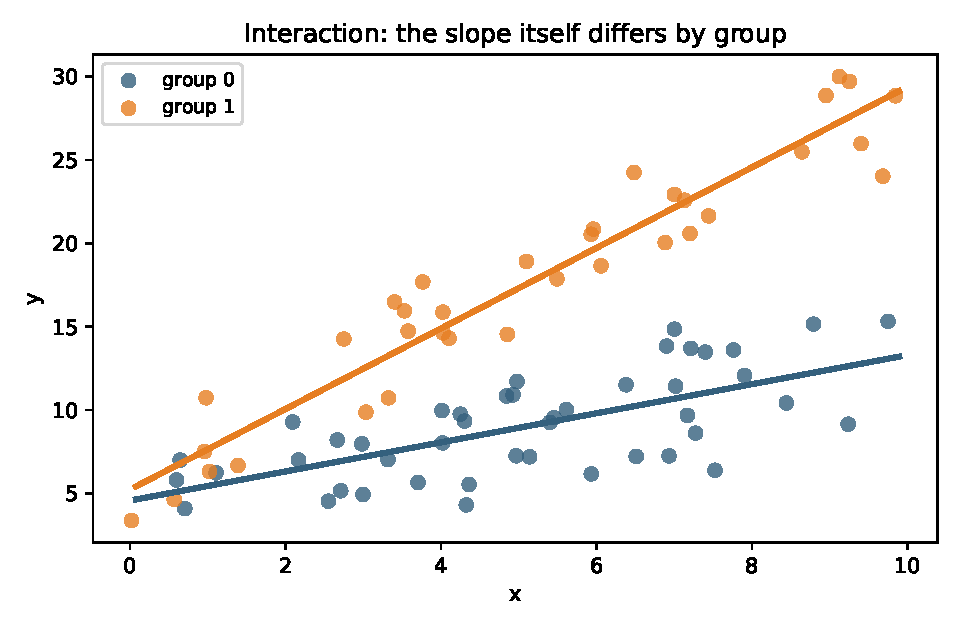
\includegraphics[width=\textwidth]{fig_interaction.pdf}
\end{column}
\begin{column}{0.44\textwidth}
\small
A dummy shifts the line. An \textbf{interaction} (a $\text{group}\times x$ term) lets the
\emph{slope} change too.
\begin{itemize}
  \item Lines are no longer parallel.
  \item Now ``the effect of $x$'' depends on the group.
\end{itemize}
We'll go deeper on interactions in Part 3.
\end{column}
\end{columns}
\end{frame}

\begin{frame}{Your turn \#2}
\begin{yourturn}{interpret the coefficient}
A model of monthly rent gives
\[
   \widehat{\text{rent}} = 600 + 0.9\,(\text{sqft}) + 250\,(\text{has parking}),
\]
where \emph{has parking} is 1 if yes, 0 if no.
\vspace{0.2em}
Practice explaining to a neighbor what the \textbf{250} means. Be careful to say what is being
held fixed.
\end{yourturn}
\end{frame}

\begin{frame}{Your turn \#2: answer}
\begin{itemize}
  \item ``Among units \emph{of the same size}, having parking is associated with about
        \textbf{\$250 more} rent per month.''
  \item The phrase ``of the same size'' is the whole point: the coefficient holds square
        footage fixed. Drop that phrase and you've changed the claim.
\end{itemize}
\begin{principle}{coefficients are conditional}
Every coefficient in a multi-predictor model means ``holding the other predictors fixed.''
Saying that phrase out loud is what separates a correct interpretation from a wrong one.
\end{principle}
\end{frame}

% ======================================================================
\section{Confounding}
% ======================================================================
\begin{frame}{Multiple regression, quickly}
With more than one predictor,
\[
   \hat{y} = b_0 + b_1 x_1 + b_2 x_2 + \dots + b_k x_k ,
\]
\begin{itemize}
  \item each coefficient is the effect of \emph{its} predictor \textbf{holding all the others
        fixed}.
  \item That little phrase is where all the statistical thinking lives. The same slope can look
        completely different depending on what else is in the model.
\end{itemize}
\begin{principle}{marginal vs.\ partial}
A slope with $x$ alone (marginal) and the same slope with other variables added (partial) are
answers to \emph{different questions}. Neither is ``the truth'' on its own.
\end{principle}
\end{frame}

\begin{frame}{Confounding: a lurking variable pulls the strings}
\begin{itemize}
  \item A \textbf{confounder} is a third variable that drives both $x$ and $y$.
  \item It can manufacture a relationship that isn't really about $x$ at all, or hide one that
        is.
  \item Example: ice cream sales predict drowning deaths. Not because ice cream is dangerous,
        but because \emph{summer} drives both.
\end{itemize}
\begin{principle}{the question to always ask}
Before trusting a slope as ``the effect of $x$,'' ask: what else moves with $x$ that also moves
$y$? That third variable is where slopes go to die.
\end{principle}
\end{frame}

\begin{frame}{Your turn \#3 (vote)}
\begin{yourturn}{predict the within-group slope}
A health study finds that, across everyone, \textbf{more weekly exercise} goes with
\textbf{higher cholesterol}: a clearly positive slope.
\vspace{0.4em}

Now we split people by \textbf{age group} and look \emph{within} each one. Vote:
\vspace{0.2em}
\begin{center}
\textbf{(A)} still positive \qquad \textbf{(B)} flat \qquad \textbf{(C)} flips negative
\end{center}
\end{yourturn}
\end{frame}

\begin{frame}{The reveal: same data, opposite story}
\begin{columns}[c]
\begin{column}{0.66\textwidth}
\centering
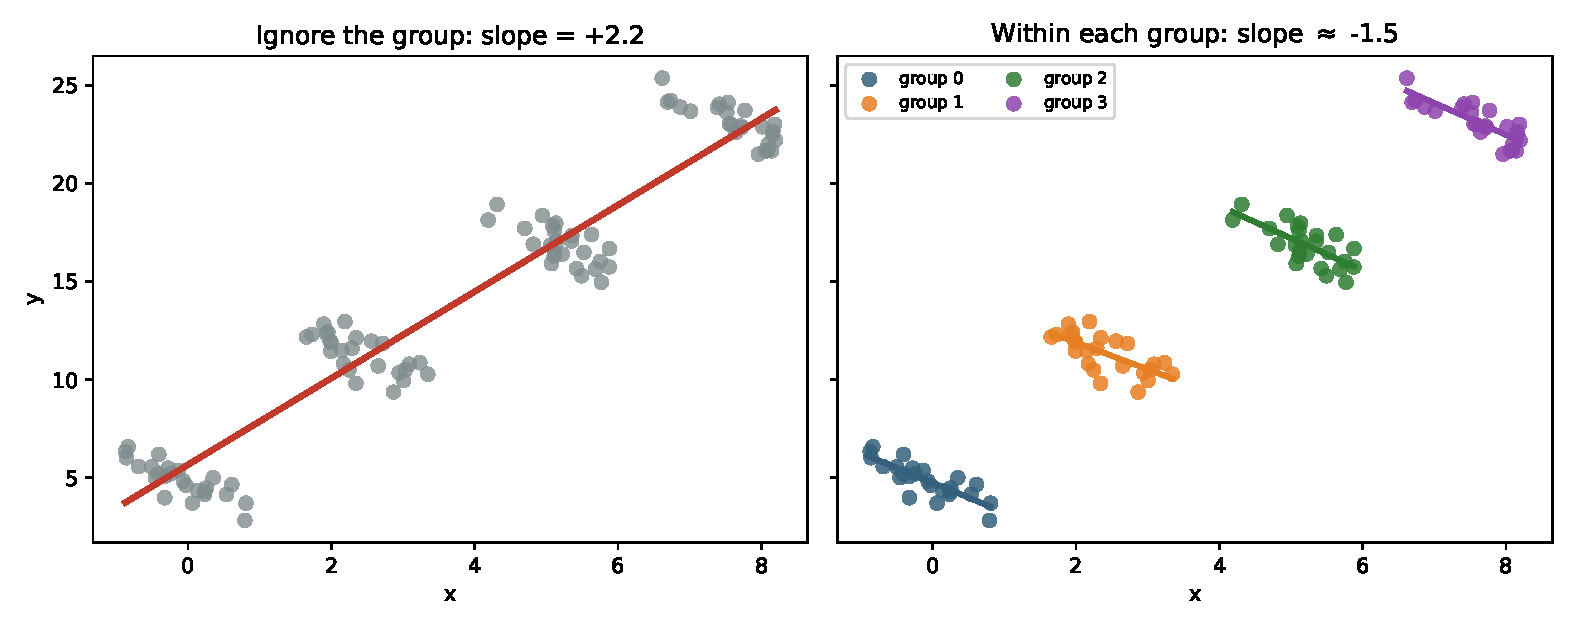
\includegraphics[width=\textwidth]{fig_confounding.pdf}
\end{column}
\begin{column}{0.34\textwidth}
\small
Ignore age: slope is \textbf{positive} ($\approx +2.2$).
\vspace{0.4em}

Within each age group: slope is \textbf{negative} ($\approx -1.5$). Exercise lowers
cholesterol, but older people both exercise more and run higher.
\vspace{0.4em}

This sign flip is \textbf{Simpson's paradox}. Age was the confounder all along.
\end{column}
\end{columns}
\end{frame}

\begin{frame}{Adding a predictor: sometimes a fix, sometimes a wound}
\begin{itemize}
  \item Adding a \textbf{confounder} (like age above) removes bias. The slope you get after
        controlling for it answers a cleaner question.
  \item But adding the \emph{wrong} variable can create bias: a \textbf{mediator} (a step on
        the path from $x$ to $y$) or a \textbf{collider} (something $x$ and $y$ both cause).
\end{itemize}
\begin{trap}{``control for everything'' is not a strategy}
Throwing every available variable into the model can fix confounding or cause new bias,
depending on each variable's role. You need a reason for each one, not a reflex.
\end{trap}
\end{frame}

\begin{frame}{Removing a predictor: omitted-variable bias}
\begin{itemize}
  \item Leave a real confounder out and its influence doesn't vanish. It gets absorbed into the
        slopes of whatever predictors remain.
  \item That is \textbf{omitted-variable bias}: the slope you report is contaminated by the
        variable you didn't include.
  \item This is why coefficients move, sometimes dramatically, when you add or drop a single
        variable.
\end{itemize}
\begin{practice}{a classic}
``A coefficient flipped sign when I added one variable. Which is right?'' Answer: ``Whichever
model controls for the actual confounders. The sign flip is the model telling you a confounder
was hiding in the first version.''
\end{practice}
\end{frame}

\begin{frame}{Correlation is not causation, stated precisely}
\begin{itemize}
  \item A regression slope is a \textbf{description}: how $y$ moves with $x$ in this data.
  \item It becomes a \textbf{causal} statement only under an assumption you bring from outside:
        that there are no lurking confounders.
  \item Randomized experiments (like our Coke test) earn that assumption by design.
        Observational data does not.
\end{itemize}
\begin{principle}{where causation comes from}
Causation is not something a slope proves. It comes from the \emph{design} of how the data was
collected, or from assumptions you state and defend.
\end{principle}
\end{frame}

\begin{frame}{Scenario: ``does X cause Y?''}
\textbf{Setup.} A dashboard shows: users who get the onboarding email spend 20\% more. A PM
says ``the email causes more spending, send it to everyone.''
\begin{itemize}
  \item Who \emph{gets} the email may already differ: more engaged users may opt in, and
        engaged users spend more anyway. That's a confounder.
  \item The clean answer is an experiment: randomly send the email to half.
\end{itemize}
\begin{interview}{how to answer}
``The 20\% is a correlation that could be confounded by who opts in. Before claiming the email
causes spending, I'd run a randomized test, or at least control for engagement and check
whether the gap survives.''
\end{interview}
\end{frame}

\begin{frame}{From question to answer: a worked example}
\textbf{Problem.} A landlord asks: ``does adding parking really raise the rent I can charge, or
do parking units just happen to be bigger?'' Walk the six steps:
\begin{enumerate}\small
  \item \textbf{Question:} the \emph{effect} of parking on rent (explanation), not prediction.
  \item \textbf{Data:} rent, square footage, parking (0/1), one row per unit, all observed
        (nothing was randomly assigned).
  \item \textbf{Look:} parking units do tend to be larger, so size is a likely confounder.
  \item \textbf{Model:} regress rent on parking \emph{and} size, so parking is read at a fixed size.
  \item \textbf{Check:} residuals look fine, and no single building drives the result.
  \item \textbf{Answer:} ``about +\$250 holding size fixed,'' with its CI, plus the caveat that
        this is observational, so an unmeasured confounder could still remain.
\end{enumerate}
\end{frame}

% ======================================================================
\section{LLM check}
% ======================================================================
\begin{frame}{LLM check: mistake or not? (1 of 2)}
\begin{llmcheck}{we asked an LLM to interpret a regression}
\textbf{We told it:} ``Here is a regression of salary on years of education, from survey data.
Interpret it.''\\[4pt]
\textbf{It answered:} ``Each extra year of education \emph{causes} about \$4{,}200 more salary,
so requiring more schooling would raise incomes.''
\end{llmcheck}
\vspace{0.2em}
\centering\small Mistake, or no mistake? Decide before we click.
\onslide<2->{%
\begin{trap}{verdict: mistake}
Survey data is observational, so ``causes'' is unearned. Ability, family background, and field
all confound education and salary, and the policy claim rides on that bad causal leap.
\end{trap}}
\end{frame}

\begin{frame}{LLM check: mistake or not? (2 of 2)}
\begin{llmcheck}{same idea, a different answer}
\textbf{We told it:} ``Interpret the coefficient on bedrooms in a house-price model that also
includes square footage.''\\[4pt]
\textbf{It answered:} ``Holding square footage fixed, each extra bedroom is associated with
about \$9{,}000 higher predicted price. This is associational, not necessarily causal.''
\end{llmcheck}
\vspace{0.2em}
\centering\small Mistake, or no mistake?
\onslide<2->{%
\begin{principle}{verdict: no mistake}
This one is right: it holds the other predictor fixed, says ``associated'' instead of
``causes,'' and flags the causal caveat. Don't assume the model is always wrong.
\end{principle}}
\end{frame}

% ======================================================================
\section{Consolidate}
% ======================================================================
\begin{frame}{Fitting and reading a regression}
\small
\begin{enumerate}
  \item \textbf{Plot $y$ against $x$ first.} A line on a curved cloud is a wrong answer with a good $p$-value.
  \item \textbf{Fit it:} \texttt{sm.OLS(y, sm.add\_constant(X)).fit()}, then read \texttt{.summary()}.
  \item \textbf{Read the slope with its units}, and rescale to something a human feels (per 1{,}000 lbs, not per lb).
  \item \textbf{Check the slope against its SE}, which is the same estimate-over-noise ratio as always.
  \item \textbf{Get the interval}, \texttt{.conf\_int()}, and report it rather than the $p$-value alone.
  \item \textbf{Plot residuals against fitted values} to check the straight-line and constant-spread assumptions.
  \item \textbf{State the range of $x$ the data covers}, and refuse to predict outside it.
\end{enumerate}
\end{frame}

\begin{frame}{The traps, all in one place}
\begin{trap}{the ones that bite most often}
\begin{itemize}
  \item Reading a slope with no units, no direction, no uncertainty.
  \item Treating $R^2$ as the score: high means good, low means useless.
  \item Confusing a significant slope with an important one.
  \item Interpreting a coefficient without saying ``holding the others fixed.''
  \item Forgetting which level is the categorical baseline.
  \item Calling a slope ``the effect'' while a confounder is lurking.
  \item Controlling for everything, including mediators and colliders, on reflex.
  \item Reading an observational slope as proof of causation.
\end{itemize}
\end{trap}
\end{frame}

\begin{frame}{Ten questions to be able to answer}
\begin{enumerate}\small
  \item What does the slope mean, in the units of this problem?
  \item Our slope is significant but $R^2$ is 0.04. Is the model useful?
  \item How do you put a categorical predictor with five levels into a regression?
  \item What does an interaction term mean, in plain language?
  \item The coefficient flipped sign when we added a variable. What happened?
  \item When is controlling for a variable the right move, and when is it a mistake?
  \item Can you say the slope is the effect of changing $x$? Under what conditions?
  \item Two predictors are highly correlated. What happens to their coefficients?
  \item How would you explain a regression output to a non-technical manager?
  \item What would make you distrust a regression you did not run yourself?
\end{enumerate}
\end{frame}

\begin{frame}{Mastery checklist}
You have this unit when you can, from memory:
\begin{itemize}
  \item state any slope as a sentence with units, direction, and uncertainty
  \item test a slope and explain its $p$-value and CI in plain words
  \item separate significance, effect size, and $R^2$
  \item interpret dummy and categorical coefficients against their baseline
  \item explain what ``holding the others fixed'' does to a coefficient
  \item recognize confounding, and explain why adding or removing a variable moves slopes
  \item say exactly when a slope is causal and when it is only a description
  \item walk a regression analysis from question to answer in the right order
\end{itemize}
\end{frame}

\begin{frame}{How to read any regression coefficient}
\begin{principle}{the reusable structure}
\begin{enumerate}
  \item \textbf{Say the sentence:} ``each extra (unit of $x$) is associated with $b$ more
        (units of $y$), holding the other predictors fixed.''
  \item \textbf{Add the uncertainty:} the SE and the confidence interval.
  \item \textbf{Separate} significance, size, and $R^2$. They answer different questions.
  \item \textbf{Ask what's missing:} which confounder could be moving this slope?
  \item \textbf{Decide:} description or causal claim, and is the design strong enough to say so?
\end{enumerate}
\end{principle}
\centering
That structure works for a coffee chain, a rent model, or a neural network's last layer.
\end{frame}

\begin{frame}{What you should be able to do with software}
\small
Nobody is asking you to memorize syntax. You are expected to know \emph{which} procedure the
question calls for, what to hand it, and what the output means. With an AI assistant open, you
should be able to produce any of these and defend the result.
\begin{center}\footnotesize
\begin{tabular}{p{0.44\textwidth} p{0.46\textwidth}}
\toprule
\textbf{You should be able to} & \textbf{What you would reach for} \\
\midrule
Simple and multiple regression & \texttt{sm.OLS(y, sm.add\_constant(X)).fit()} \\
Formula interface with categories & \texttt{smf.ols(\"y \textasciitilde\ x + C(group)\", data)} \\
An interaction & \texttt{smf.ols(\"y \textasciitilde\ x * group\", data)} \\
Coefficient intervals & \texttt{fit.conf\_int()} \\
Residual diagnostics & \texttt{fit.resid} against \texttt{fit.fittedvalues} \\
Correlation between predictors & \texttt{df[cols].corr()} \\
Transform a skewed variable & \texttt{np.log(y)}, then interpret on the log scale \\
\bottomrule
\end{tabular}
\end{center}
\vspace{0.2em}
\centering\small
If you cannot say what the output means, the fact that you produced it is worth nothing.
\end{frame}

\begin{frame}{Where we go next}
\begin{itemize}
  \item We held the model fixed and read one slope at a time. \textbf{Part 3} is about
        \emph{building} the model: several predictors at once, interactions, transformations,
        and the constant tension between fitting the data and overfitting it.
  \item The thread continues: every coefficient is still an estimate with uncertainty, and the
        hardest questions are still about which variables belong.
\end{itemize}
\begin{principle}{the through-line}
A model is a set of answers, one per coefficient. Your job is to know which question each one
answers, and which variable might be quietly changing the answer.
\end{principle}
\end{frame}

\end{document}
